\documentclass[11pt]{article}
\usepackage[margin=2.2cm]{geometry}
\usepackage{fontspec}
\setmainfont{STIX Two Text}
\setmonofont{Menlo}[Scale=0.85]
\newfontfamily\symfont{STIX Two Math}
\usepackage[russian,english]{babel}
\usepackage{graphicx,booktabs,tabularx,float,caption,amsmath,amssymb}
\captionsetup{font=small}
\setlength{\parskip}{4pt}\setlength{\parindent}{0pt}
\begin{document}
\selectlanguage{russian}
{\LARGE\bfseries Когда условной генеративной модели можно верить как постериору: идентифицируемость, полоса сглаживания и OOF-перекалибровка\par}\bigskip

*Черновик ML-статьи в читаемом виде, 19 сентября 2026 (вечер). Всё, что уже посчитано, — с числами и ссылками на файлы; чего нет — помечено «[ЭКСПЕРИМЕНТА ЕЩЁ НЕТ]» с указанием, что и когда планируется. Английский LaTeX-вариант: \texttt{docs/paper/main.tex}.*

\bigskip\hrule\bigskip

\section*{Аннотация}

Сэмплы условных диффузионных и flow-matching моделей всё чаще читают как выборку из постериора: ансамбли погоды, реконструкции в обратных задачах, анализы в ассимиляции данных. Одни такие ансамбли калиброваны (GenCast), многие — нет. Мы даём простое объяснение. Условная flow-matching модель, обученная на парах «условие {\symfont →} одна реализация», — это непараметрическая оценка условной плотности с неявной \emph{полосой сглаживания по условию}: она воспроизводит p(y|x) только если обучающие условия плотны на масштабе, где p(y|x) ещё не меняется. Если условие идентифицирует свою единственную реализацию, эмпирический минимизатор \emph{любого} strictly proper objective — точечная масса (Теорема 1); разброс модели — артефакт полосы, сжимающийся с обучением. Мы доказываем, что свежий шум на условии превращает population-минимизатор в точный байесовский постериор при эмпирическом прайоре, т.е. в оценку Надарая–Ватсона с полосой σ (Теорема 2); отсюда критерий «калибровка, когда σ превышает расстояние до соседа» и цена — информация. Мы показываем, что копула смеси реальных реализаций сходится к истинной (Теорема 3), и это лицензия на перекалибровку маргиналов с сохранением копулы генератора. Контролируемые эксперименты с известным постериором подтверждают каждое утверждение, включая тест на изображениях. В операционной задаче ассимиляции морского льда с реальной геометрией спутниковых треков, где у условий доказуемо нет соседей (шесть независимых лет), перекалиброванный ансамбль калиброван на dev-годе (CRPS {\symfont −}19 \% к лучшему стандартному baseline'у, spread/skill .99, плоские rank-гистограммы, верные атомы) и без перенастройки переносится на запечатанный test-год из 200 дней подряд (CRPS {\symfont −}44 \%, spread/skill .98, 189/200 дней), а модель без идентифицирующей части условия калибрована по построению ценой 10 \% skill.

\bigskip\hrule\bigskip

\section*{1. Введение}

Условные генеративные модели в population-limit переносят шум ровно в p(y|x) (Lipman et al., 2023). На практике их обучают на конечных данных, где на каждое условие x\_i приходится \textbf{одна} реализация y\_i: одно будущее на каждое начальное состояние, одно изображение на каждое измерение, один анализ на каждый фон. Ансамбль, полученный многократным сэмплированием, читают как постериор. Для GenCast (Price et al., 2025) это чтение верно; для многих других систем — включая модель ассимиляции морского льда, с которой мы начали, — нет: её ансамбль был недодисперсен на постоянный множитель во всех режимах, а разброс \emph{монотонно падал} с обучением.

Наше объяснение элементарно. Обученная сеть конечной ёмкости действует на условие как сглаживатель: её закон в новом x — взвешенная смесь обучающих реализаций \emph{соседних} условий. Когда соседи есть на масштабе, где p(y|x) не меняется (58 000 начальных состояний с гладким хаотическим откликом, как у GenCast), смесь и есть правильное распределение. Когда условие идентифицирует свою реализацию — фон, встречающийся один раз; измерение, служащее отпечатком изображения, — соседей нет, эмпирический минимизатор есть точечная масса, а наблюдаемый разброс — ширина окна сглаживания сети, которое закрывается по мере обучения. Замена objective не помогает: у всех strictly proper objective один минимизатор.

\textbf{Вклады.} (i) Формализация: Теорема 1 (точечная масса), Теорема 2 (шум на условии = постериор при эмпирическом прайоре = явная полоса), Теорема 3 (копула смеси). (ii) Контролируемые эксперименты с известным постериором: плотность условий, шум как полоса, «три закона», копула, учитель–ученик на изображениях. (iii) OOF-перекалибровка из классических блоков (kriging невязок, OOF-квантили по ячейкам, ensemble copula coupling) с гарантией калибровки относительно σ-алгебры ячеек. (iv) Реальный кейс с диагнозом и причинными вмешательствами.

\bigskip\hrule\bigskip

\section*{2. Постановка и взгляд «сеть = сглаживатель»}

Условие x, цель y {\symfont ∈} ℝ\^\{\}m, закон p(y|x). CFM учит поле скорости v\_θ(y\_t, x, t), минимизируя E‖v\_θ(y\_t, x\_i, t) {\symfont −} (y\_i {\symfont −} y\_0)‖², y\_t = (1{\symfont −}t)y\_0 + t·y\_i, y\_0 \textasciitilde\{\} N(0, I), и сэмплирует интегрированием ẏ = v\_θ. В population-limit минимизатор порождает p(·|x) (Lipman et al., 2023). Ничего в этом утверждении не касается конечной выборки \emph{по оси условия} — а именно там решается калибровка.

\textbf{Теорема 1 (точечная масса).} Пусть S — strictly proper scoring rule, условие x\_i встречается в выборке один раз с ответом y\_i, класс моделей не ограничен в x\_i. Тогда единственный минимизатор эмпирического риска в x\_i есть δ\_\{y\_i\}. Для CFM минимизирующее поле в x\_i — поле единственной пары (y\_0, y\_i), чей поток переносит N(0, I) в δ\_\{y\_i\}. \emph{Доказательство:} вклад точки i — S(Q(·|x\_i), y\_i) = E\_\{Y\textasciitilde\{\}δ\_\{y\_i\}\} S(Q, Y), минимизируется единственно при Q = δ\_\{y\_i\} по определению strict properness. Для CFM: v* = E[y\_i {\symfont −} y\_0 | y\_t] при фиксированном y\_i (Lipman, Thm. 1 при p\_1 = δ). {\symfont ∎} \emph{Интуиция:} студент, видевший каждый билет один раз с ответом, отвечает на новый билет смесью ответов на похожие; его «неуверенность» — ширина смеси, а не знание о задаче, и чем лучше он различает билеты, тем уже смесь.

\textbf{Идеализация сглаживателя.} Q\_θ(·|x) {\symfont ≈} Σ\_i w\_h(x, x\_i) δ\_\{y\_i\} с полосой h, убывающей с обучением. Для location-scale семейства y = μ(x) + s(x)z: Cov[Q\_θ(·|x)] = Σ\_i w\_i s(x\_i)² Σ{\symfont ₀} + Σ\_i w\_i (μ(x\_i) {\symfont −} μ̄)(μ(x\_i) {\symfont −} μ̄)\textsuperscript{T}, {\symfont →} истинная ковариация при плотных соседях, {\symfont →} 0 при N\_h = Σw\_i / max w\_i {\symfont →} 1. Разброс модели — разброс истин соседей, свойство плотности обучающей выборки, а не p(y|x). Для сети без явного шума это \textbf{гипотеза} (доказана только при явном шуме — Теорема 2; NTK-рассуждения не переносятся автоматически на закон решения ODE — это замечание ревью, мы его приняли).

\textbf{Теорема 2 (шум на условии — явная полоса).} Пусть пары порождаются так: i \textasciitilde\{\} Unif, ε \textasciitilde\{\} N(0, σ²I) свежий на каждом шаге, x̃ = x\_i + ε, y = y\_i; v\_σ — минимизатор population-CFM-objective относительно закона P\_σ этих пар. Тогда поток v\_σ(·, x̃, ·) переносит N(0, I) в Q\_σ(·|x̃) = Σ\_i w\_i(x̃) δ\_\{y\_i\}, w\_i {\symfont ∝} φ\_σ(x̃ {\symfont −} x\_i). \emph{Доказательство:} P\_σ имеет плотность по x̃ и условный закон Σ w\_i δ\_\{y\_i\} по формуле Байеса; условная CFM-теорема к P\_σ. Свежий шум гарантирует несмещённость стохастического градиента относительно P\_σ. {\symfont ∎} \textbf{Следствия.} (a) Q\_σ — оценка Надарая–Ватсона с полосой σ, независимо от архитектуры. (b) Q\_σ — \emph{в точности} постериор при наблюдении x̃ и эмпирическом прайоре (1/N)Σδ\_\{(x\_i,y\_i)\}: модель калибрована для \emph{зашумлённой} задачи по построению, с её резкостью. (c) Состоятельность для истинного p(y|x) при N {\symfont →} {\symfont ∞}, σ {\symfont →} 0, Nσ\^\{\}d {\symfont →} {\symfont ∞}; при конечном N эффективное число соседей N\_σ = Σw\_i/max w\_i, и при σ {\symfont ≪} d\_NN — Теорема 1 «через заднюю дверь»; d\_NN \textasciitilde\{\} N\^\{\}\{{\symfont −}1/d\} — проклятие размерности. (d) Фиксированный (не пересэмплируемый) шум делает x̃\_i детерминированной функцией i — не помогает. (e) \textbf{Смешивание только вдоль зашумлённых координат}: если x = (b, o) и шум только на o, а b (фон, \emph{маска наблюдений}, любой идентификатор) точен и уникален, то Q\_σ(·|b\_i, õ) = δ\_\{y\_i\}. \textbf{Замечание.} Теорема 2 описывает \emph{цель} аугментированной задачи, не закон конечной сети: сеть добавляет собственное сглаживание и может оказаться ближе к истинному постериору, чем сама цель (§3.3). Одна реализация на условие не исключает оценки в параметрических/гладких классах (Tang et al., 2024); наше утверждение — о режиме, где p(y|x) не разрешается условиями на масштабе их шага.

\textbf{Теорема 3 (копула смеси).} Пусть p(·|x) — закон y = μ(x) + s(x)z, z \textasciitilde\{\} F с непрерывными маргиналами и копулой C, не зависящей от x; Q(·|x) = Σ w\_i p(·|x\_i), Δ = Σ w\_i(‖μ(x\_i) {\symfont −} μ(x)‖ + |s(x\_i) {\symfont −} s(x)|)/s\_min. Тогда ‖C\_Q {\symfont −} C‖\_{\symfont ∞} {\symfont →} 0 при Δ {\symfont →} 0; для гауссовой F — {\symfont ≤} c{\symfont √}Δ. \emph{Набросок:} KL смеси {\symfont ≤} Σ w\_i KL\_i (выпуклость), TV {\symfont ≤} {\symfont √}(KL/2), непрерывность оператора Склара при сходимости совместных законов с непрерывными маргиналами. {\symfont ∎} \textbf{Оговорка (по ревью).} Теорема 3 — о смеси реальных реализаций \emph{до} коллапса; она не говорит, какова копула сколлапсировавшей сети (N(0, ε²R\_ρ) {\symfont →} δ{\symfont ₀} при любой ρ — сжатие масштаба не определяет копулу). Операционное утверждение слабее и проверяемо: ошибка генератора преимущественно маргинальная, а его зависимость полезнее стационарной модели или зависимости чужой даты (§5.6).

\bigskip\hrule\bigskip

\section*{3. Контролируемые эксперименты (истина известна)}

Условие x \textasciitilde\{\} U[{\symfont −}1,1]², цель y {\symfont ∈} ℝ¹{\symfont ⁶}, y|x \textasciitilde\{\} N(f(x), σ(x)²K), f — гладкие случайные фурье-признаки, σ(x) гетероскедастична, K экспоненциальная. Ученик — MLP-CFM (3×256), 20k шагов Adam, Euler-32, 32 члена. Разброс сравнивается с истинной σ, ранги — с истинным законом, energy score — со свежими истинными выборками.

\textbf{3.1 Плотность, а не число реализаций} (\texttt{synth\_realizations\_per\_condition.json}). При фиксированном бюджете N·k = 2048 число реализаций на условие k не важно (spread/σ .92–.95 при k = 1…16). При фиксированном N = 512 модель с k = 1 коллапсирует с обучением (.92 {\symfont →} .81, rank-TV .06 {\symfont →} .15, OOS RMSE растёт .079 {\symfont →} .101), с k = 16 — стоит на .95. При N = 8192 и k = 1 — 1.00.

\begin{figure}[H]\centering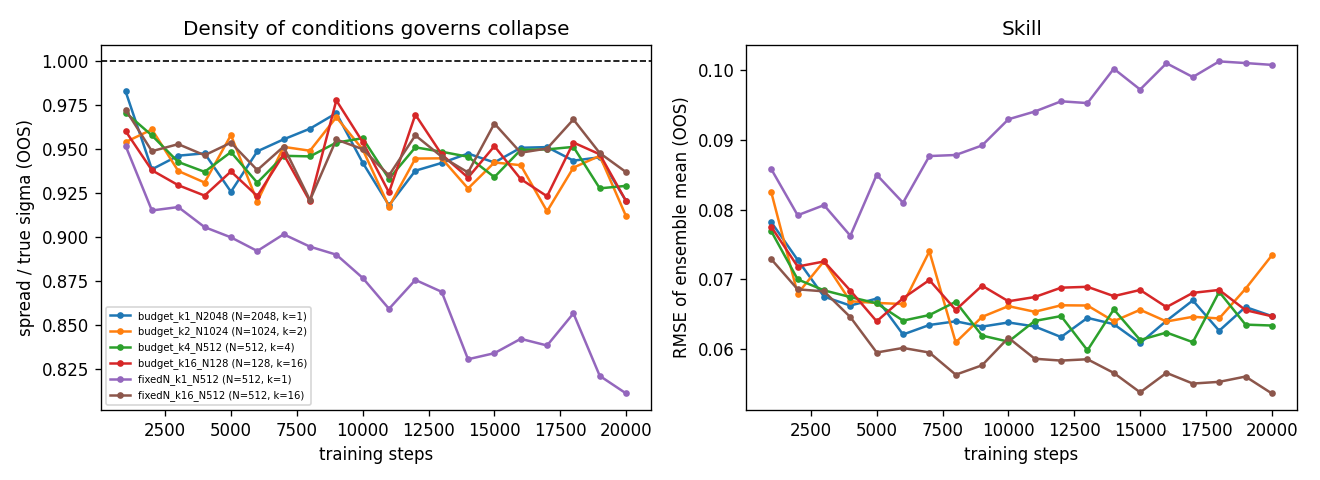
\includegraphics[width=\textwidth]{../research/figures/fig_synth_realizations.png}\caption*{Плотность условий против числа реализаций (слева) и сохранение копулы при коллапсе (справа).}\end{figure}

\begin{figure}[H]\centering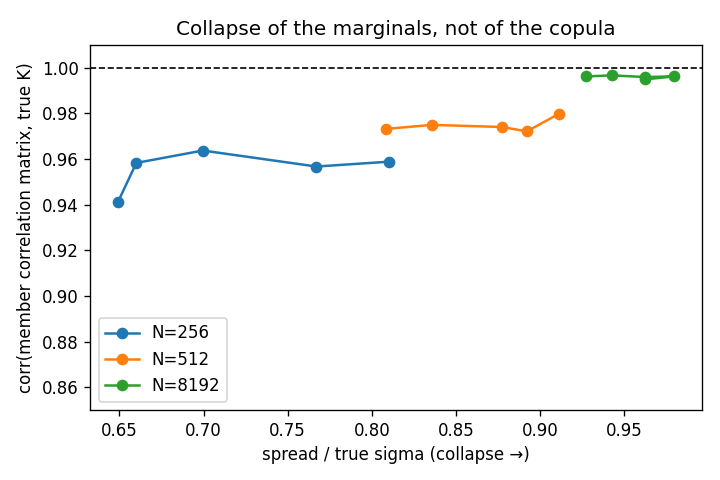
\includegraphics[width=\textwidth]{../research/figures/fig_synth_copula.png}\caption*{Копула переживает коллапс маргиналов: корреляция корреляционной матрицы членов с истинной K против spread/σ.}\end{figure}

\textbf{3.2 Шум — это полоса} (\texttt{synth\_noisy\_partial\_obs\_v3.json}). Условие = 6 зашумлённых координат цели (латент не даётся), истинный постериор считается точно на сетке (сходимость сетки 81 {\symfont →} 161 проверена: разница средних .004). Таблица spread/σ\_true после 20k шагов:

\begin{center}\footnotesize\begin{tabularx}{\textwidth}{lXXXX}\toprule
N & d\_NN & σ = 0 & σ = .1 & σ = .3 \\ \midrule
512 & .19 & \textbf{.24} (коллапс) & .62 & \textbf{.96} \\
2048 & .14 & .81 & .91 & .99 \\
8192 & .11 & \textbf{1.00} & 1.00 & 1.00 \\
\bottomrule\end{tabularx}\end{center}

Калибровка при σ {\symfont ≳} d\_NN или при плотных условиях; при σ = .3 модель {\symfont ≈} точный постериор зашумлённой задачи (ES .90 = истинный .90); цена — оптимальный RMSE растёт .23 {\symfont →} .37. Фиксированный шум (v1) не помогает ни при каком σ. Случайные маски из 8008 паттернов (v2) — не выучивается даже среднее: предупреждение о размерности условия.

\begin{figure}[H]\centering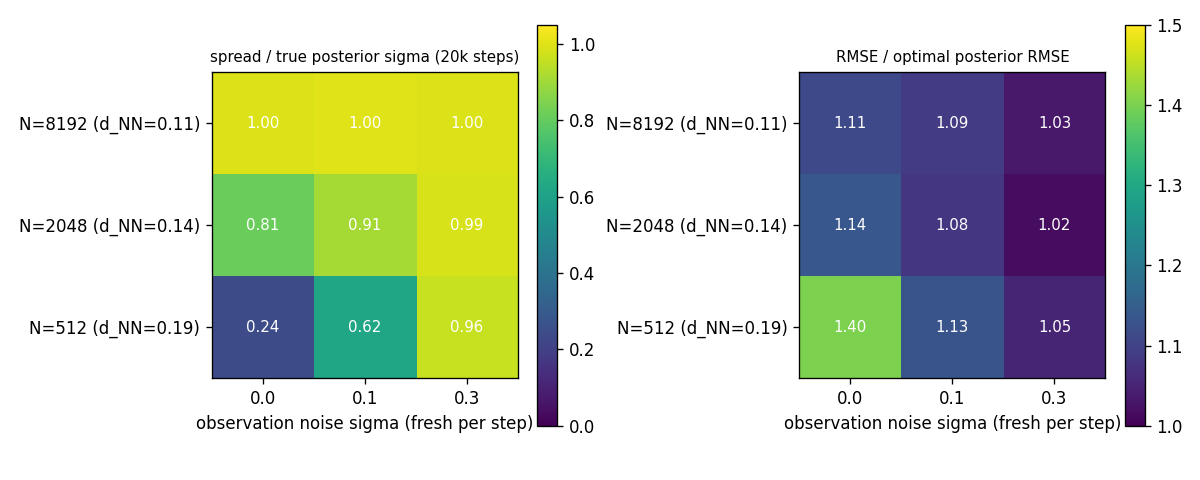
\includegraphics[width=\textwidth]{../research/figures/fig_synth_noise_bandwidth.png}\caption*{Условие = зашумлённые координаты цели: spread/σ истинного постериора и RMSE/оптимум как функции N (с расстоянием до соседа d\_NN) и σ.}\end{figure}

\textbf{3.3 «Три закона»} (\texttt{synth\_three\_laws.json}; по требованию ревью). На 96 держанных условиях: истинный постериор P*, эмпирическая аугментированная смесь P̂\_\{D,σ\} (цель Теоремы 2, сэмплируется без обучения), точное CFM-поле смеси через Euler-32 (ODE-ошибка), сеть Q\_θ.

\begin{center}\footnotesize\begin{tabularx}{\textwidth}{lXXXXXX}\toprule
N & σ & закон & spread/σ* & RMSE ср. & ES (P*: ref) & rank-TV \\ \midrule
512 & .1 & смесь / ODE(смесь) / \textbf{сеть} & .57 / .59 / \textbf{.61} & .289 / .284 / \textbf{.158} & 1.25 / 1.23 / \textbf{.79} (.55) & .63 / .63 / \textbf{.27} \\
512 & .3 & смесь / ODE / сеть & .97 / .96 / .95 & .17 / .17 / .14 & 1.09 / 1.10 / .97 (.91) & .15 / .15 / .11 \\
2048 & .1 & смесь / ODE / \textbf{сеть} & .58 / .59 / \textbf{.90} & .215 / .213 / \textbf{.106} & 1.13 / 1.12 / \textbf{.68} (.65) & .56 / .53 / \textbf{.10} \\
2048 & .3 & смесь / ODE / сеть & .99 / .97 / 1.00 & .14 / .13 / .11 & 1.00 / 1.01 / .95 (.93) & .10 / .11 / .07 \\
\bottomrule\end{tabularx}\end{center}

Интегратор точен. При σ = .3 цель Теоремы 2 {\symfont ≈} истина, сеть её воспроизводит. При σ = .1 цель почти точечная (N\_eff 1.4–1.8), а сеть \textbf{лучше своей цели} — собственное сглаживание сети добавляется к σ. Теорема 2 — гарантированный «пол»; выше — индуктивное смещение, которое надо измерять; оно же и сжимается по кривой коллапса.

\textbf{3.4 Копула переживает коллапс маргиналов} (\texttt{synth\_copula\_check.json}). При k = 1, N = 256 spread/σ падает .81 {\symfont →} .65 за обучение, а корреляция корреляционной матрицы членов с истинной K остаётся .96 {\symfont →} .94; при N = 8192 — .99 {\symfont →} 1.00.

\textbf{3.5 Изображения: учитель–ученик} (\texttt{teacher\_student\_mnist.json}, фигура \texttt{fig\_mnist\_teacher\_student.png}). Процедурный учитель: условие (класс MNIST, поворот θ {\symfont ∈} [{\symfont −}45°, 45°], масштаб s {\symfont ∈} [.8, 1.2]); p(y|x) = случайный экземпляр класса, повёрнутый и масштабированный, + пиксельный шум — истинный постериор сэмплируется. Ученик — FiLM-UNet-CFM, 15k шагов, 32 члена, 200 держанных условий.

\begin{center}\footnotesize\begin{tabularx}{\textwidth}{lXXXX}\toprule
плечо & spread/true & RMSE ср. & ES (истина) & rank-TV \\ \midrule
N = 500, k = 1 & \textbf{.38} & .19 & 6.85 (4.23) & .48 \\
N = 2000, k = 1 & .85 & .10 & 4.55 (4.15) & .13 \\
N = 8000, k = 1 & \textbf{.92} & .06 & 4.13 (4.07) & .10 \\
N = 2000 + уникальный ключ (8-dim) в условии & \textbf{.29} & .18 & 6.59 (4.17) & .29 \\
ключ + свежий шум σ = .5 & .64 & .13 & 5.12 (4.18) & .19 \\
ключ + свежий шум σ = 1.0 & \textbf{.82} & .10 & 4.50 (4.13) & .13 \\
ключ, k = 8 реализаций на ключ & \textbf{.95} & .06 & 4.15 (4.07) & .10 \\
\bottomrule\end{tabularx}\end{center}

Плотность управляет коллапсом и на изображениях; идентификатор при том же N вызывает коллапс; свежий шум на ключе возвращает калибровку по мере роста σ; при 8 реализациях на ключ идентификатор безвреден. Это Теоремы 1–2 на данных, которые ML-сообщество считает своими.

\begin{figure}[H]\centering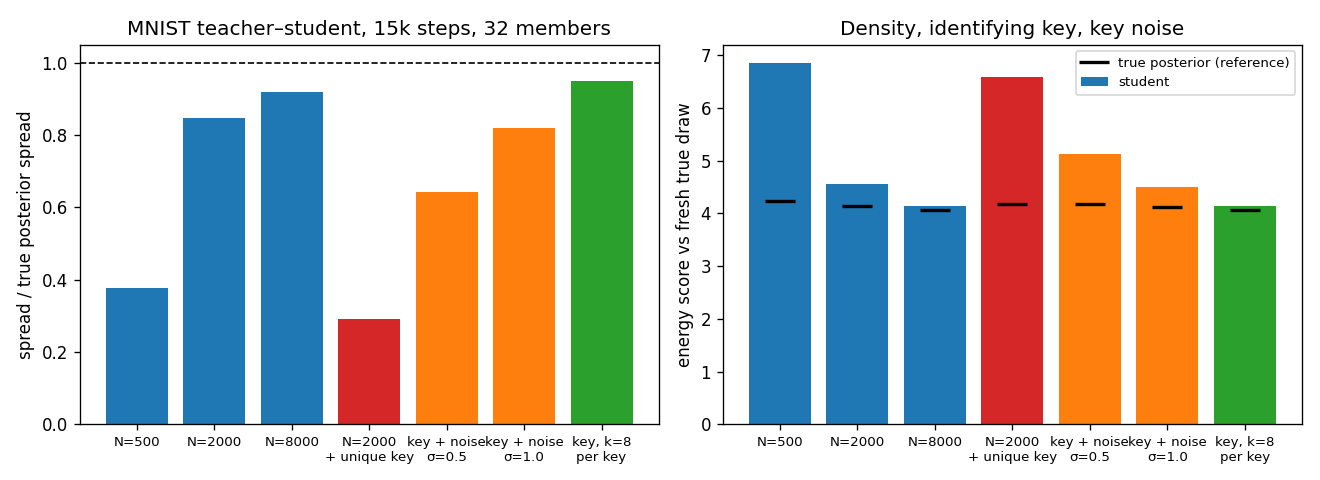
\includegraphics[width=\textwidth]{../research/figures/fig_mnist_teacher_student.png}\caption*{MNIST учитель–ученик: плотность условий (синие), уникальный ключ {\symfont →} коллапс (красный), свежий шум на ключе {\symfont →} восстановление (оранжевые), 8 реализаций на ключ (зелёный).}\end{figure}

\textbf{[ЭКСПЕРИМЕНТА ЕЩЁ НЕТ]} Чистый тест ключа в дизайне ревью (16 категорий × 128 ответов, фиксированный vs пересэмплируемый ключ) — покрыт плечами MNIST «ключ / ключ + шум / k = 8», отдельная категориальная версия не делалась. \textbf{[ЭКСПЕРИМЕНТА ЕЩЁ НЕТ]} Второй физический домен с МК-истиной (2-D турбулентность с управляемым числом реализаций) — план после закрытия ледового блока (\textasciitilde\{\}неделя).

\bigskip\hrule\bigskip

\section*{4. OOF-перекалибровка (метод)}

Если генератор даёт условное среднее и правдоподобную копулу, но артефактный разброс, Теоремы 1–3 подсказывают декомпозицию: маргиналы — заново, вне выборки; копулу — от генератора. Реализация для полей с атомами (ровно 0, cap) и разреженными точными наблюдениями:

\begin{itemize}\item \textbf{Латент с атомами.} Вода {\symfont →} {\symfont −}γ·(расстояние до кромки), cap {\symfont →} цензурирование; атомы становятся пороговыми событиями непрерывного латента.\item \textbf{Условное среднее.} Латент среднего генератора обновляется kriging'ом невязок треков obs {\symfont −} μ (стационарный двухмасштабный прайор, ядро OOF, per-date nugget по leave-one-out на невязках самого дня); наблюдения дня d соблюдаются точно.\item \textbf{Маргиналы.} Остаток truth {\symfont −} μ{\symfont ₂} описывается эмпирическими квантилями по ячейкам (расстояние до трека дня d × значение μ{\symfont ₂}), оценёнными на \emph{других} датах (5 фолдов, purge ±1).\item \textbf{Копула.} Член k получает гауссов скор {\symfont √}½·ã\_k + {\symfont √}½·g\_k, где ã\_k — стандартизованный по пикселю паттерн аномалии генератора, g\_k — независимое стационарное поле только длинного масштаба; PIT смешанного скора — эмпирическая по ячейкам \emph{внутри даты} (без истины); u {\symfont →} квантили ячейки.\end{itemize}

\textbf{Гарантии (Proposition).} (a) Пулированный по членам маргинал в каждой ячейке — OOF-закон ячейки точно (внутридатная PIT; аудит: KS .000–.005); по членам — с отклонением .01–.02, потому что члены генератора не одинаково распределены (масштаб аномалий .75–.89). (b) При λ \textgreater\{\} 0 члены обменяемы, но не независимы (стандартизация связывает их) — fair scores оптимистичны; мы дополнительно считаем cross-score по двум независимо обработанным банкам. (c) При обмениваемости дат внутри ячеек OOF-квантильные полосы имеют конечно-выборочное маргинальное покрытие (split-conformal); ансамбль auto-калиброван относительно σ-алгебры ячеек и есть единственный минимизатор ожидаемого proper score в классе законов, измеримых относительно ячеек. (d) Резкость ограничена информацией ячеек. Связь с EMOS, ECC, GCA (Gneiting 2005; Schefzik 2013; Möller 2013) прямая; новое — \emph{почему} это работает для генеративного ансамбля (Теорема 3) и OOF-конструкция маргиналов на самих оцениваемых датах.

\textbf{История версий (честно).} v3 {\symfont →} v15 отбирались по score на тех же 40 датах (оптимизм отбора \textasciitilde\{\}4 \% CRPS между v9–v15); v16 {\symfont →} v19 — исправления корректности PIT без изменения score. Отвергнуто с числами: cap-порог (масса чинится, различение нет), режимные ячейки по невязке дня, глобальный и block-CV nugget, чистая копула генератора (v12: 40/40 дат по fair CRPS, но U-ранги при s/r 1.1 — члены не обменяемы; поучительный пример, как proper score переоценивает, а ранги ловят), сезонные ячейки на одном годе.

\bigskip\hrule\bigskip

\section*{5. Реальный кейс: ассимиляция морского льда}

\textbf{5.1 Задача.} Анализ концентрации (и толщины) льда дня d на арктической подобласти 320×256 из фона — поля модели той же даты \textbf{прошлого года} — и наблюдений на реальных треках Sentinel-3 SRAL дней d, d{\symfont −}1, d{\symfont −}2 (OSSE: значения — модельная истина на реальной геометрии; \textasciitilde\{\}700 px/день, \textasciitilde\{\}150 пунктирных сегментов, только юг области). Генератор — UNet 50M concat-CFM, обучение 2016–2021, dev — 40 дат 2022 (10 членов), test — 2023 (один прогон). Протоколы: native (толщина видна) и siconc-only (толщина скрыта, для сравнения с 3D-Var).

\textbf{5.2 Нет соседей.} Доминирующая неопределённость при данном фоне — межгодовая аномалия (73 \% дисперсии крупномасштабной аномалии объясняется парой год–месяц), реализаций — шесть. Измерено: для 40 dev-дат расстояние от фона до ближайшего обучающего фона (2170 фонов, крупный масштаб) = .47 медианно от RMS аномалии, которую надо предсказать; сосед часто из другого месяца. Это режим коллапса из §3.

\textbf{5.3 Коллапс и константный разброс.} Чистая CFM-модель: val\_loss {\symfont ↑} после эп. 5, OOS RMSE {\symfont ↑} после эп. 7, разброс монотонно {\symfont ↓} (s/RMSE .68 {\symfont →} .43); под строгим протоколом s/r .49, cov80 .31. Модель с 50 \% безусловных шагов не коллапсирует, но её разброс — константа выборки (.135–.141 во всех четырёх клетках «год × протокол») при ошибке .156–.190; in-sample тест опровергает запоминание. Регуляризованное переобучение (dropout условий, ранняя остановка) даёт s/r .98 ценой +6 \% RMSE.

\begin{figure}[H]\centering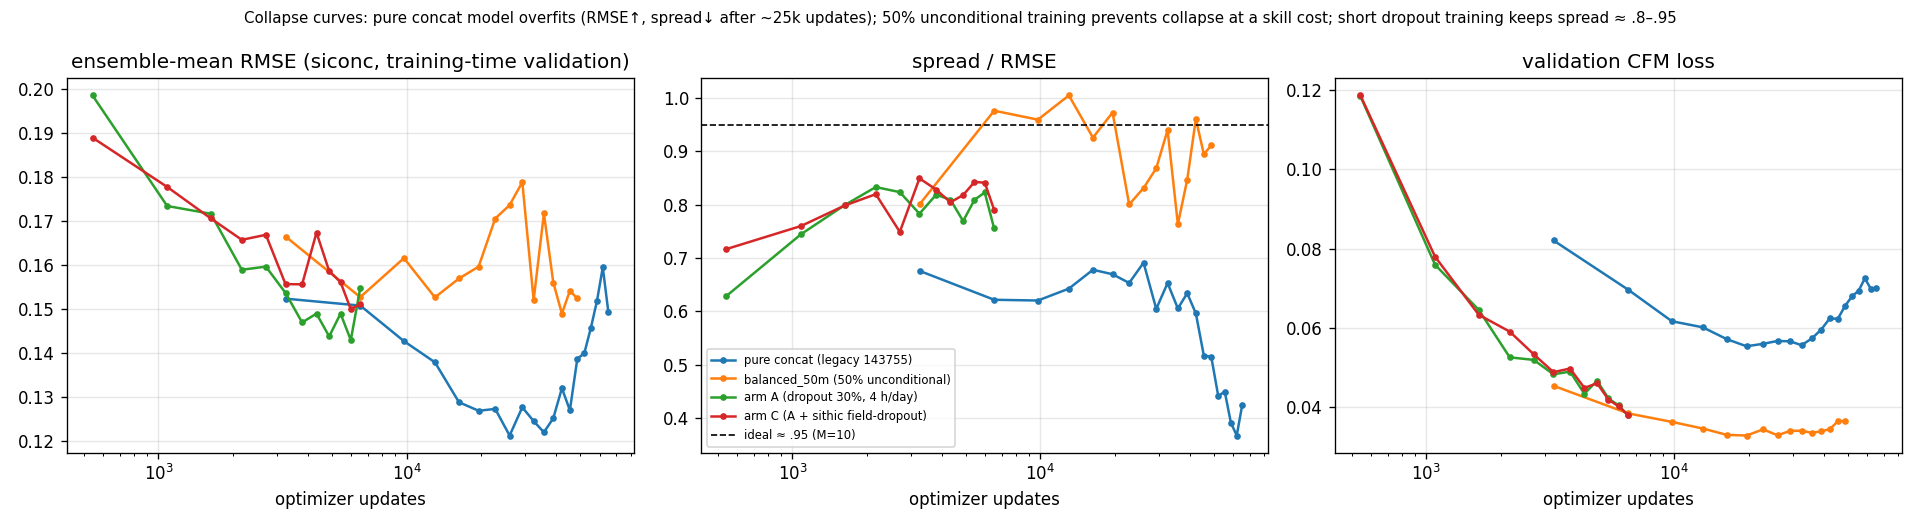
\includegraphics[width=\textwidth]{../research/figures/fig_collapse_curves.png}\caption*{Кривые обучения: val\_loss, OOS RMSE среднего и spread/RMSE чистой CFM-модели (коллапс) и модели с 50 \% безусловных шагов.}\end{figure}

\textbf{5.4 Перекалиброванный ансамбль (OOS, dev-2022, native).} Слой v19 поверх balanced-генератора, cross-fit: fair CRPS .0415 {\symfont →} \textbf{.0337} ({\symfont −}19 \%, 39/40 дат), RMSE .156 {\symfont →} .136, s/r .99 во всех стратумах, pooled rank-TV .015 (null-допуск идеального 10-членного ансамбля .034), cov80 .81–.91, Brier атома нуля .069 {\symfont →} .037, наблюдения дня d точно. Многомерные score: ES патчей {\symfont −}17 \% (33/40), variogram на 8–32 px лучше, блочный CRPS 4/16/64 px {\symfont −}21/{\symfont −}27/{\symfont −}34 \% (39–40/40), спектр высоких волновых чисел 1.15× истины (генератор 1.11). Под siconc-only: {\symfont −}31 \% (40/40). На train-2019 (стресс): {\symfont −}32 \% в среднем, 14 зимних дат хуже raw — условное смещение генератора сезонное (зимой {\symfont ≈} 0, летом {\symfont −}.1…{\symfont −}.5), пулированные ячейки переносят летний сдвиг на зиму; сезонная ось чинит среднее (31/40 дат), но тонка на одном годе.

\begin{figure}[H]\centering\includegraphics[width=\textwidth]{../research/figures/rank_hist_layer_v19.png}\caption*{Rank-гистограммы слоя v19 (пулированная и по стратумам расстояния до трека дня d).}\end{figure}

\begin{figure}[H]\centering\includegraphics[width=\textwidth]{../research/figures/fig_atom_reliability_v19.png}\caption*{Reliability атомов: ровно 0, лёд \textgreater\{\} .15, cap — генератор vs генератор + слой.}\end{figure}

\begin{figure}[H]\centering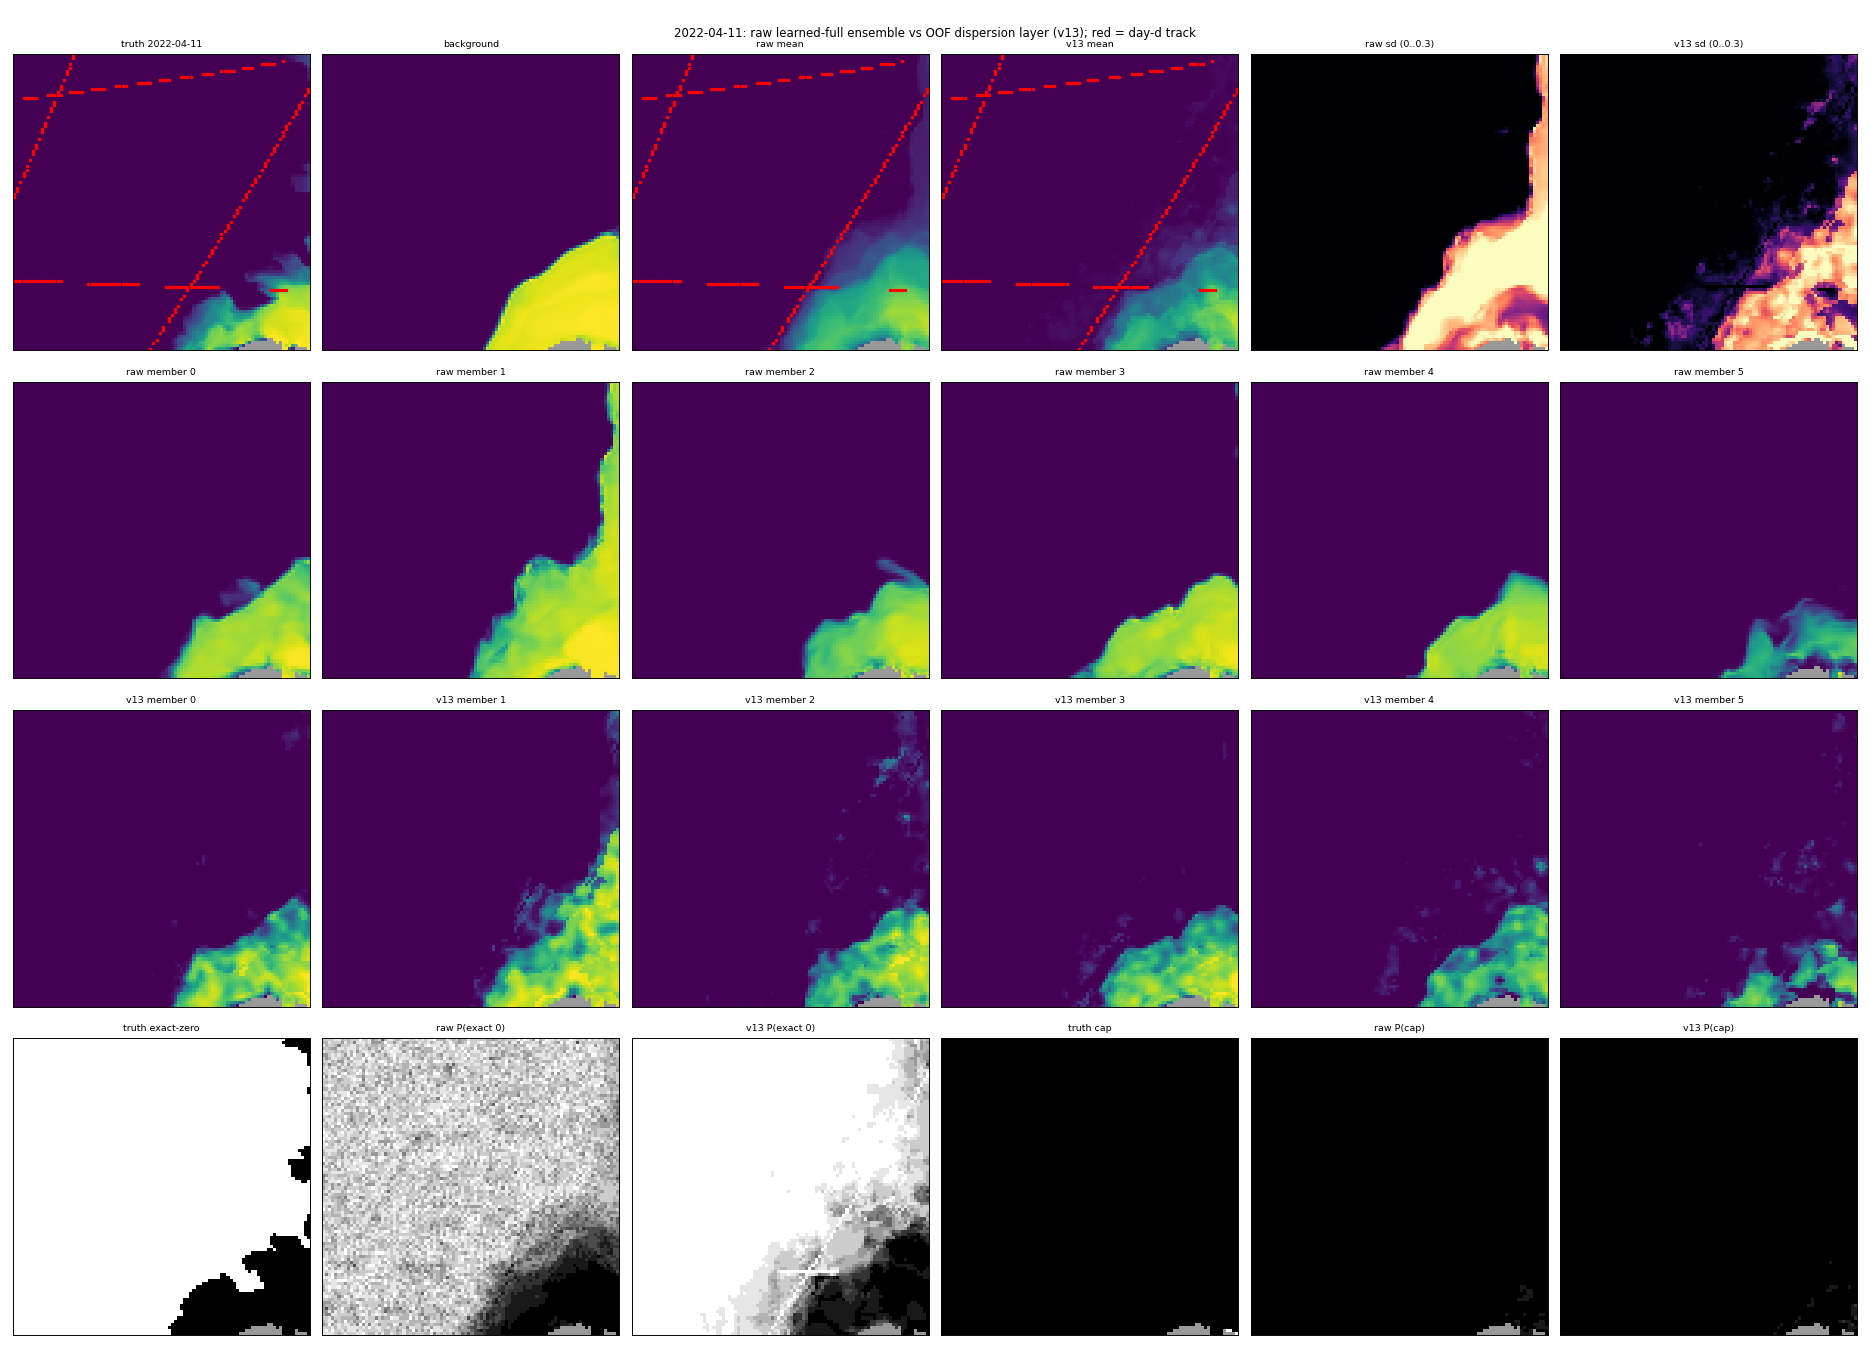
\includegraphics[width=\textwidth]{../research/figures/v13_2022-04-11_zoom.png}\caption*{Члены ансамбля 11 апреля 2022: истина, фон, сырое среднее и sd, члены генератора, члены слоя, карты P(0) и P(cap).}\end{figure}

\textbf{5.5 Откуда выигрыш (абляции при одинаковых маргиналах).}

\begin{center}\footnotesize\begin{tabularx}{\textwidth}{lXXXXX}\toprule
вариант & CRPS (дат \textless\{\} raw) & ES & VS lag 1 / 16 & ранги & s/r \\ \midrule
raw & .0415 & .821 & .0060 / .0271 & .157 & .93 \\
только среднее (kriging + obs) & .0352 (37) & \textbf{.703} & \textbf{.0058} / .0231 & .129 & .97 \\
+ маргиналы, стационарная копула & .0352 (34) & .728 & .0066 / .0254 & \textbf{.081} & .96 \\
+ маргиналы, копула генератора (своя дата) & \textbf{.0340} (40) & .725 & .0069 / .0243 & .094 & 1.16 \\
+ маргиналы, копула чужой даты & .0351 (32) & .723 & .0078 / .0244 & .093 & 1.04 \\
+ маргиналы, смесь (v15) & .0341 (38) & \textbf{.689} & .0067 / .0245 & .084 & 1.03 \\
\bottomrule\end{tabularx}\end{center}

76 \% выигрыша CRPS — детерминированный DA-апдейт среднего (kriging + наблюдения); перекалибровка даёт калибровку (ранги .13 {\symfont →} .08), не skill; копула генератора лучше стационарной и чужой даты в одноточечном CRPS, но по ES выигрывает только смесь. Честная формула: генератор даёт среднее и структуру, классическая ассимиляция — skill, OOF-маргиналы — калибровку.

\textbf{5.6 Стандартные baseline'ы постобработки} (вокруг сырого среднего, та же настройка на фолдах): EMOS-масштаб .0413, ECC-Q с теми же OOF-маргиналами .0408 (чинит нули .41 {\symfont →} .53 и cov80 .76 {\symfont →} .88, но не skill), conformal-полоса .0564. Слой .0335 — {\symfont −}19 \% к лучшему baseline'у, потому что дефект генератора — условное смещение и носитель, а не масштаб разброса.

\textbf{5.7 Аудит закона семплирования.} PIT смешанного скора: λ = 1 — KS .01–.02; λ = .5 с Φ — .05–.06 (хвосты сжаты); λ = 0 — .11–.15 (причина U-рангов v12); v19 (внутридатная PIT) — пулированно {\symfont ≈} 0. Cross-score по двум независимым банкам: .0331 против .0413 у raw (лучше на 40/40) — выигрыш не держится на предположении независимости членов; unit-test Roberts (стратифицированный ансамбль {\symfont →} fair CRPS M/[6(M+1)]) воспроизведён.

\textbf{5.8 Без генератора.} Фон + kriging + OOF-закон + стационарная копула: калиброван (s/r .93, ранги .077), но CRPS .050 против .034 с генератором; вдали от треков генератор снижает ошибку .244 {\symfont →} .197. \textbf{[ЭКСПЕРИМЕНТА ЕЩЁ НЕТ]} Детерминированный UNet-MSE с теми же каналами + слой со своей настройкой (arm R) — обучение стоит в очереди на GPU на сегодняшнюю ночь; это ответ на «нужна ли именно генеративность».

\textbf{5.9 Убираем идентифицирующую часть условия.} Arm D — та же архитектура без фона (только треки трёх дней, свежий шум σ = .05, 24 эпохи). Разброс больше не сжимается с обучением (spread .164 {\symfont →} .143 при RMSE .257 {\symfont →} .191; s/r .64 {\symfont →} .75), в отличие от чистой модели с фоном (.68 {\symfont →} .43). Под строгим протоколом (40 дат, 10 членов): RMSE .171 против .156 с фоном (сам фон .256), s/r .86, cov80 .79; \textbf{у треков калибровано} (s/r 1.00, cov80 .82, RMSE .098 vs .106 с фоном). Удаление ключа стоило 10 \% RMSE, не «климатологию»; остаточная недодисперсия — там, где условие не несёт информации и модель воспроизводит конкретные обучающие поля: реальная геометрия трека обучающей даты — сама по себе точная уникальная часть условия (Следствие (e)). Слой поверх arm D: CRPS {\symfont −}9 \% (25/40), ранги .16 {\symfont →} .11, вдали от треков хуже (нет информации). Arm E (реальная геометрия для всех сэмплов + реалистичная когерентная ошибка) хуже в целом, лучше у треков, не сошёлся за 24 эпохи. \textbf{[ЭКСПЕРИМЕНТА ЕЩЁ НЕТ]} Arm F — tracks-only с рандомизированной библиотечной геометрией для \emph{всех} сэмплов (проверка «маска как идентификатор») — в очереди после arm R.

\begin{figure}[H]\centering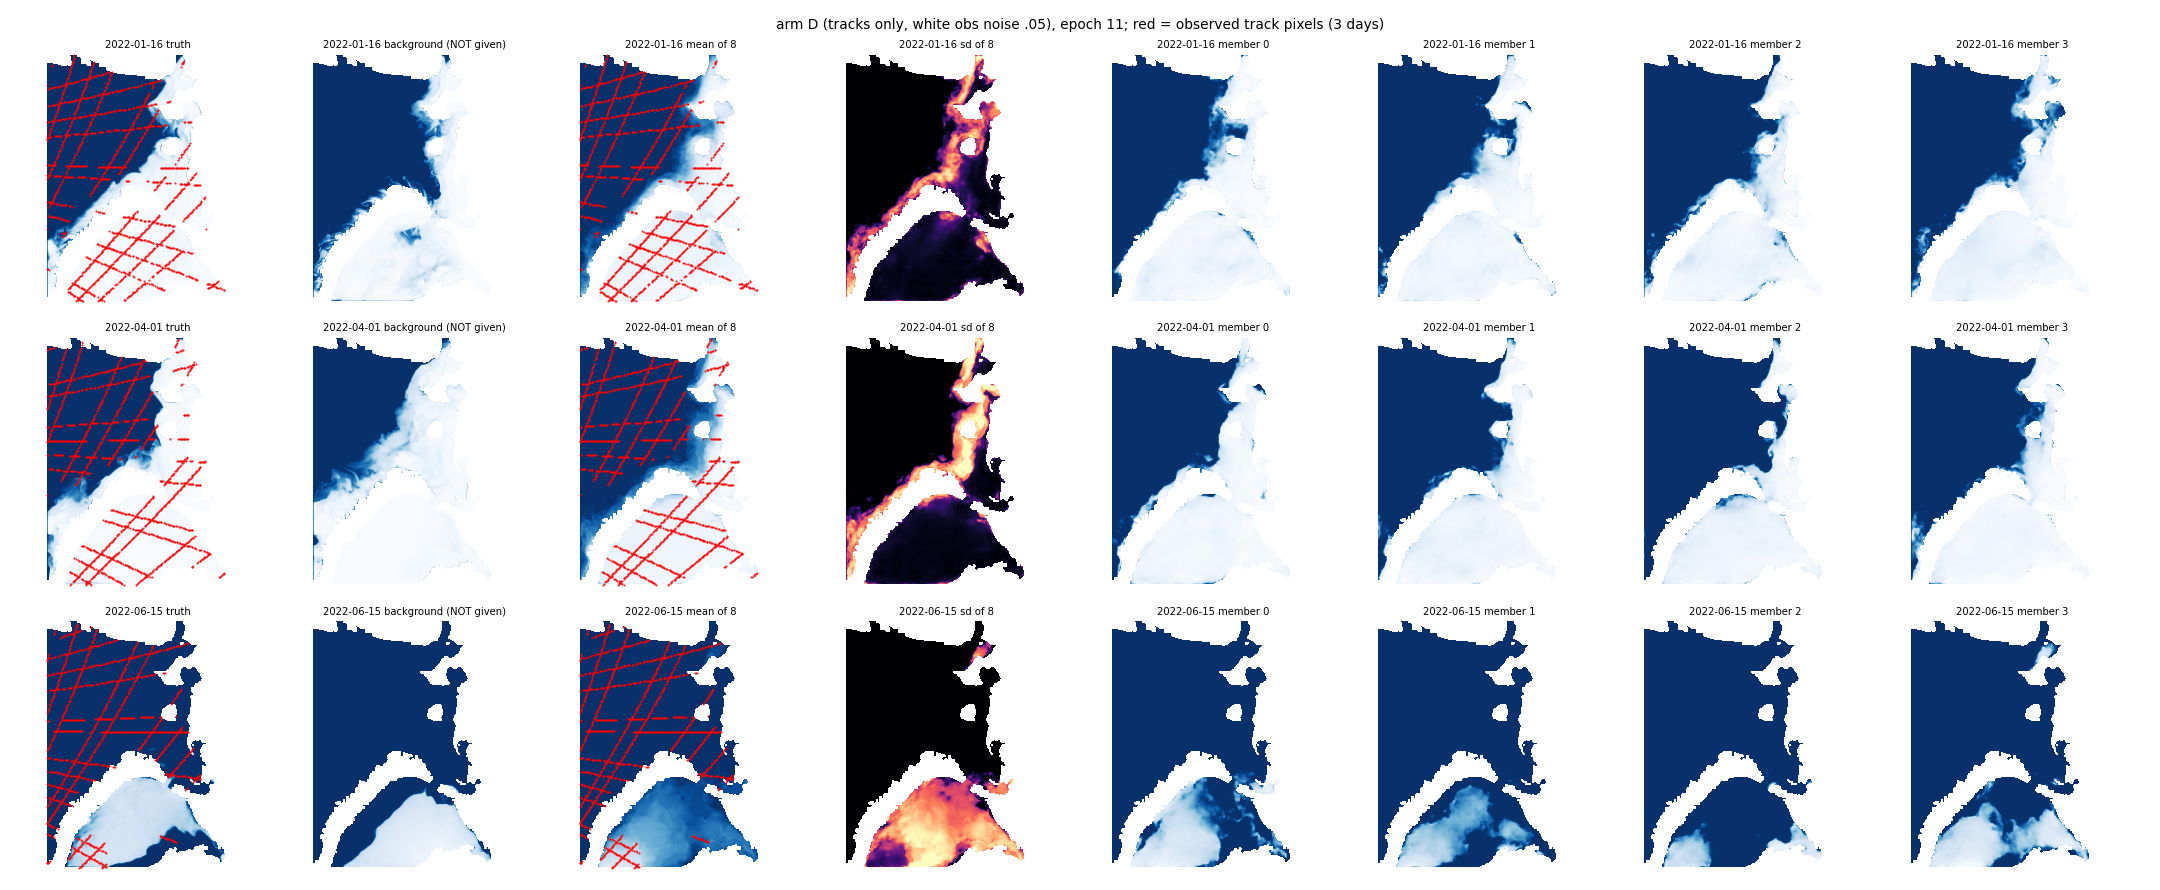
\includegraphics[width=\textwidth]{../research/figures/armD_ep0011_samples.png}\caption*{Arm D (только треки, фон не подаётся), эпоха 11: истина с треками, фон, среднее и sd по членам, четыре члена.}\end{figure}

\textbf{5.10 Реальные ошибки треков и данные.} Межпродуктовое расхождение SRAL vs AMSR2 (1461 день): sd .09 (вода) / .20–.25 (MIZ) / .11 (пак), в MIZ 64–82 \% измерений не классифицированы, ошибка когерентна вдоль трека (ρ .93/.81/.50/.06 на 1/2/4/8 px). Синтетические прямые треки прежнего OSSE покрывали всю область (север без реальных треков), четверть обучения шла без наблюдений — сделан генератор с реальной геометрией и SIC-зависимая когерентная модель ошибки. NaN в M2M = открытая вода (AMSR2 там \textasciitilde\{\}.006) — атом нуля физический.

\begin{figure}[H]\centering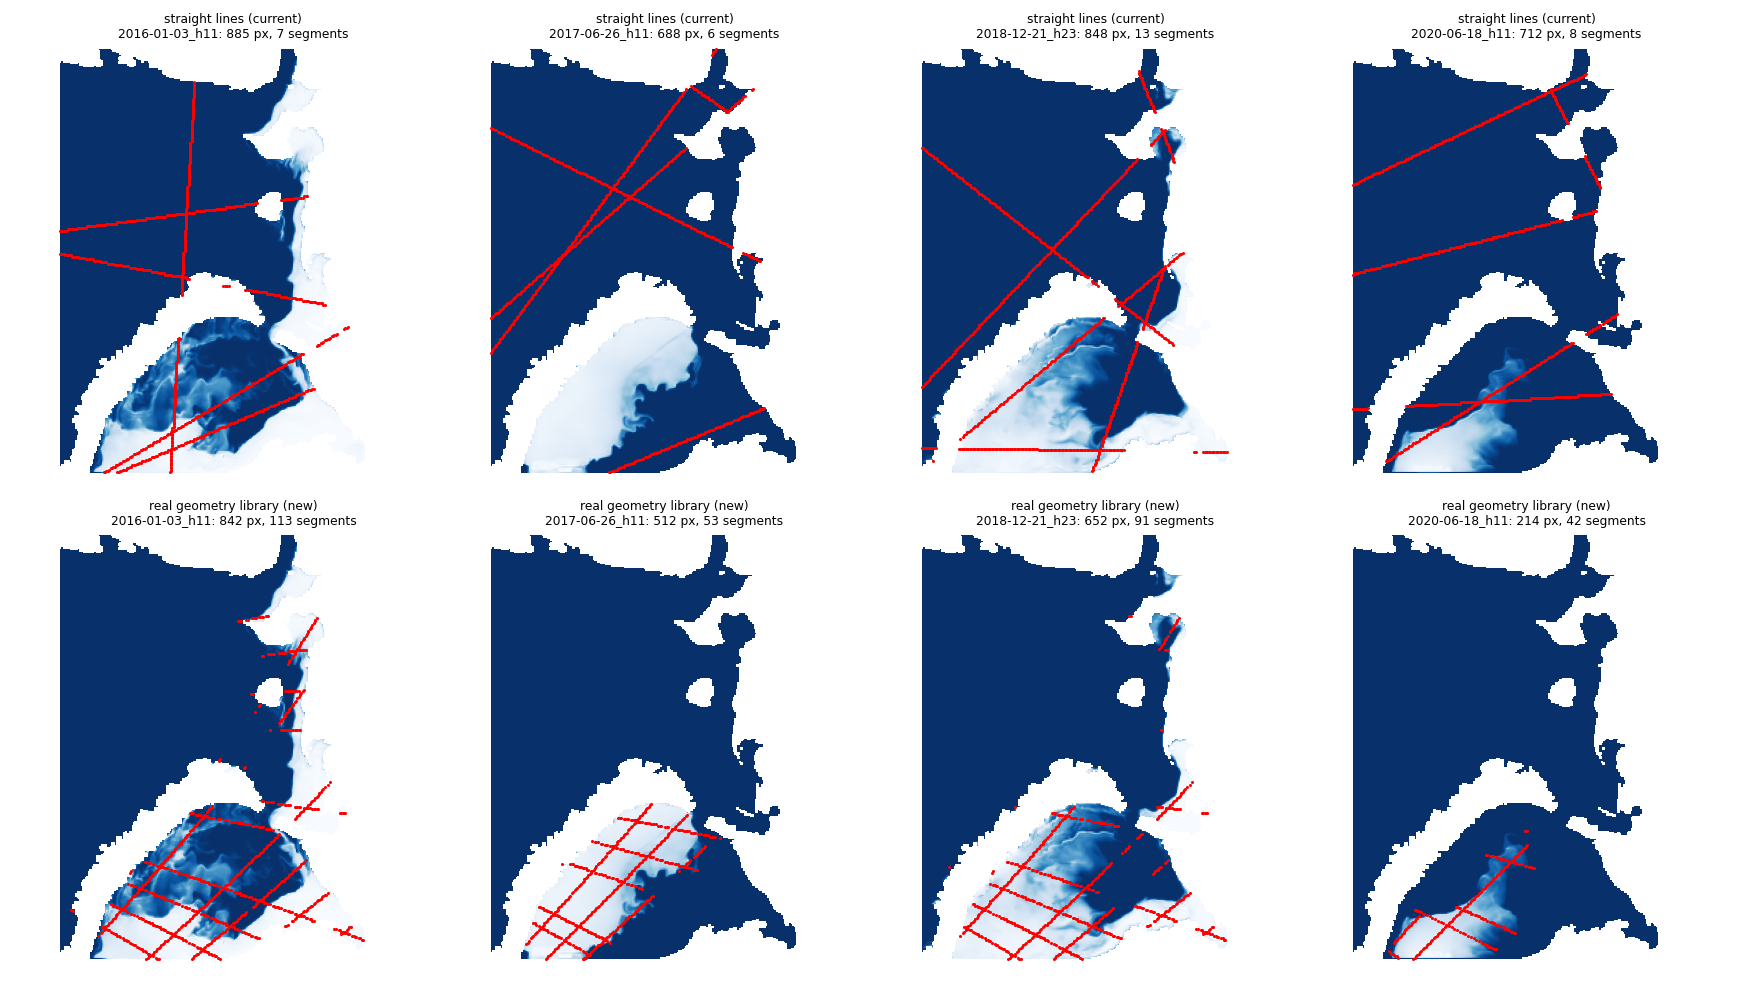
\includegraphics[width=\textwidth]{../research/figures/fig_track_geometry_straight_vs_library.png}\caption*{Синтетические прямые треки прежнего OSSE (верх) против реальной геометрии спутника из библиотеки (низ).}\end{figure}

\begin{figure}[H]\centering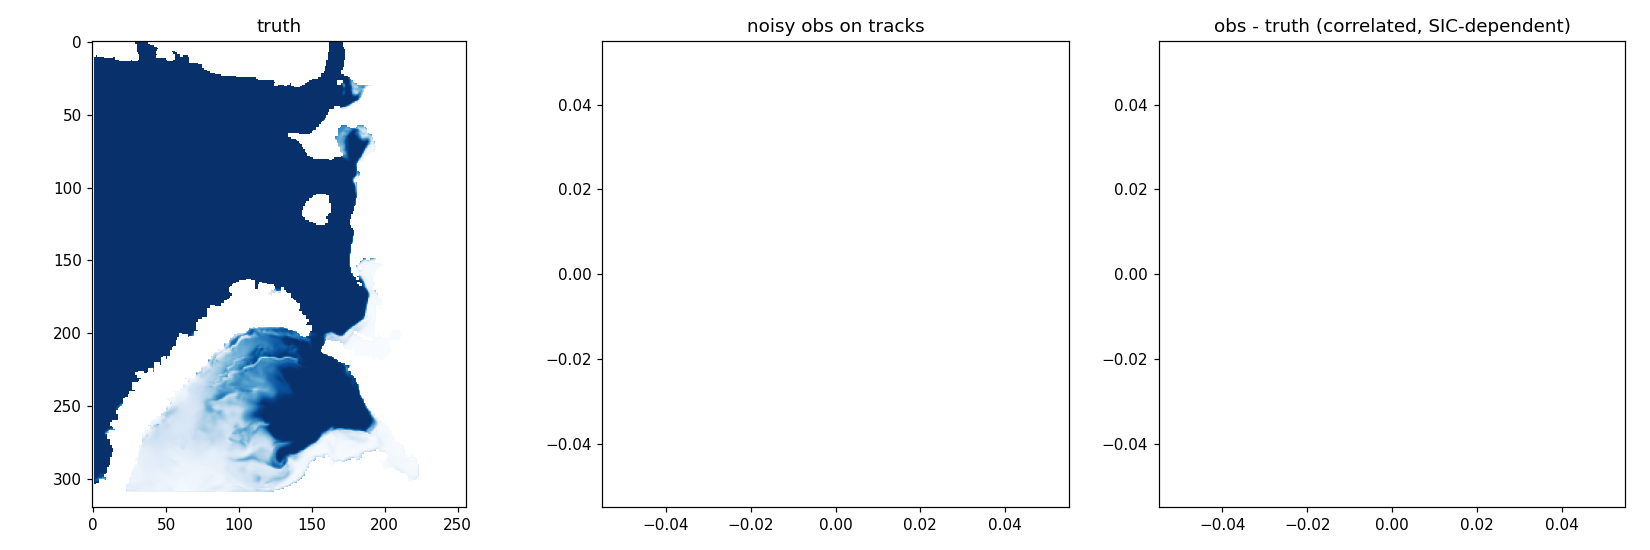
\includegraphics[width=\textwidth]{../research/figures/fig_obs_error_model.png}\caption*{Модель ошибки наблюдений: SIC-зависимая, когерентная вдоль трека (по расхождению SRAL–AMSR2).}\end{figure}

\textbf{5.11 Сравнение с 3D-Var (test-2023, 200 дней подряд, siconc-only, 5 членов).} Детерминированно, legacy-генератор: RMSE по области .275 {\symfont →} .157 (M {\symfont →} {\symfont ∞} {\symfont ≈} .144), IIEE .118 {\symfont →} .082; track\_imitation .233 {\symfont →} .098. Чистое переобучение arm C (checkpoint по dev-2022), на котором строится вероятностная строка: RMSE .275 {\symfont →} \textbf{.203} (на dev .256 {\symfont →} .181 — тот же относительный выигрыш {\symfont −}26…{\symfont −}29 \%), spread .157, s/r .87, cov80 .74, но \textbf{IIEE .118 {\symfont →} .138} — кромка в мае–июне хуже фона (.12 {\symfont →} .18, .17 {\symfont →} .26), январь–апрель как на dev. Разброс arm C между годами не изменился, а ошибка выросла: генератор «не знает», что 2023 труднее, — именно это должны чинить невязки треков дня d в слое. Вероятностная строка — единственный контакт с test: замороженный слой v19, fit \textbf{только на 40 dev-датах 2022}, применён без изменений к 200×5 сохранённым ансамблям arm C (10 членов слоя). Fair CRPS .0575 {\symfont →} \textbf{.0320} ({\symfont −}44 \%, CI95 [{\symfont −}.029, {\symfont −}.022], 189/200 дней), RMSE среднего .203 {\symfont →} \textbf{.145} (184/200; лучше детерминированного legacy .157), s/r .77 {\symfont →} \textbf{.98}, per-date rank-TV .130 {\symfont →} .067, масса нуля .46 {\symfont →} .60 (истина .63), масса cap .041 {\symfont →} .068 (истина .027 — известный перебор). По расстоянию до трека s/r 1.17 (1–2 px) … 1.05 (\textgreater\{\} 40 px). По месяцам выигрыш максимален там, где генератор был хуже всего: май CRPS .074 {\symfont →} .036, июнь .100 {\symfont →} .040 (RMSE .294 {\symfont →} .172): невязки треков дня d несут информацию о 2023, которой у генератора нет, а kriging-апдейт и OOF-маргиналы разносят её по акватории. Числа 3D-Var коллег в таблицу вставляет автор.

\begin{figure}[H]\centering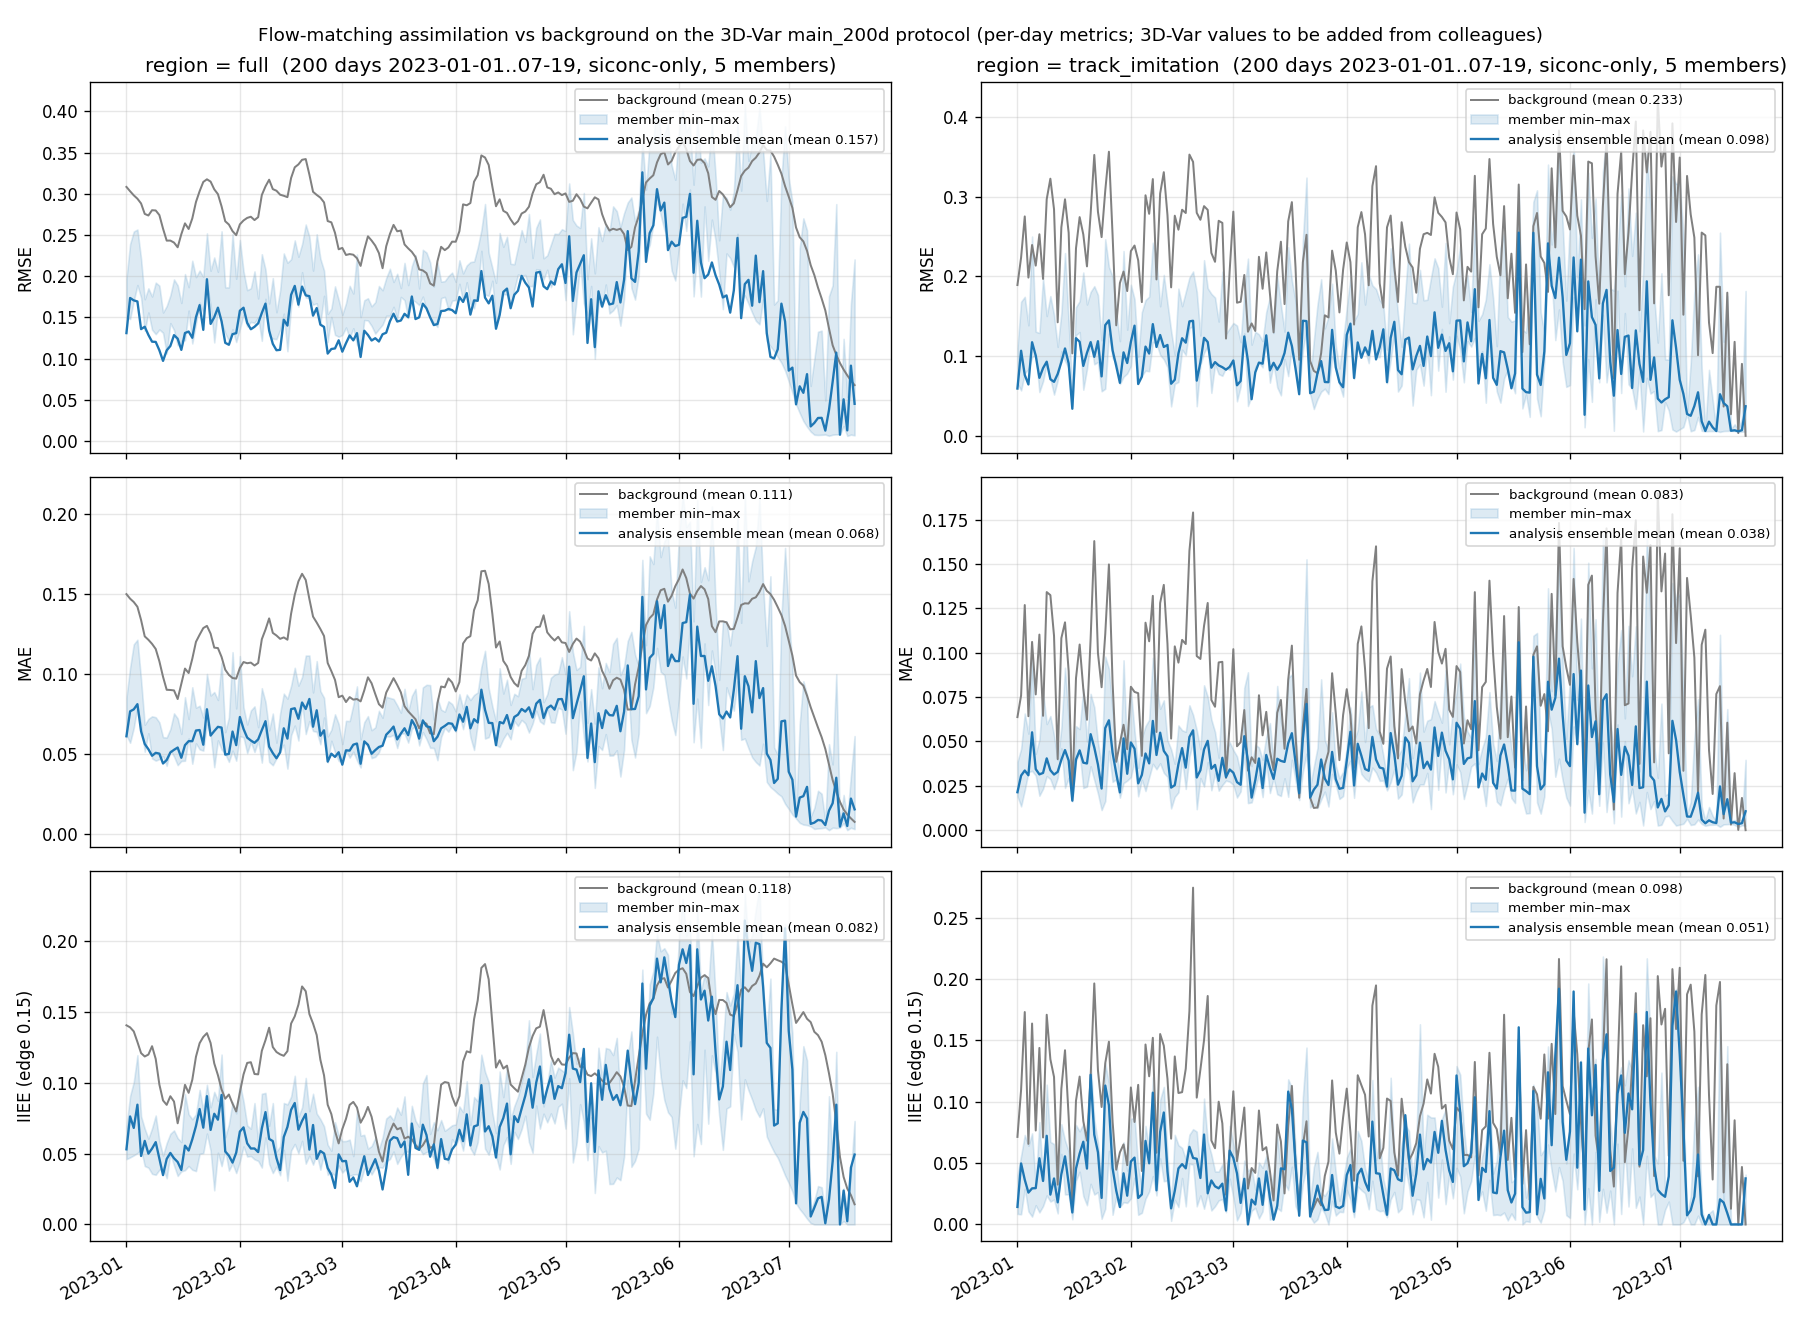
\includegraphics[width=\textwidth]{../research/figures/fig_3dvar_protocol_200d_timeseries.png}\caption*{Детерминированное сравнение по протоколу 3D-Var, 200 дней test-2023: RMSE фона и анализа по дням.}\end{figure}

\bigskip\hrule\bigskip

\section*{6. Ограничения---}

\section*{6. Ограничения}

Один OOS-год (test-2023 — второй, сегодня ночью); cap-атом не различается ни одной версией (при p \textgreater\{\} .9 частота .44); стратум \textgreater\{\} 40 px с малой статистикой; ячейки выбраны вручную, и сезонный сдвиг показывает цену пропущенного предиктора; класс копул — модель, проверяемая только многомерными score; версии слоя v3–v15 отбирались на тех же датах (оптимизм \textasciitilde\{\}4 \% CRPS; Cawley \& Talbot 2010); test-2023 уже использовался один раз для детерминированного сравнения balanced-генератора — вероятностный прогон будет вторым контактом; OSSE с точными значениями на треках против реальных SIC-зависимых когерентных ошибок и неклассифицированной MIZ; Теорема 2 — об идеальном минимизаторе, реальная сеть добавляет свою полосу; взгляд «сглаживатель» для сети без явного шума — гипотеза с одним доказанным частным случаем и эмпирикой.

\bigskip\hrule\bigskip

\section*{7. Связанные работы}

Memorization/generalization в диффузиях (Kadkhodaie et al. 2023; Yoon et al. 2023; Somepalli et al. 2023) — та же дихотомия по оси данных; у нас — по оси условия, с последствием не «воспроизведение обучающих картинок», а ложный постериор, и с условием-идентификатором, удерживающим модель в режиме запоминания при любом объёме данных. Tang et al. 2024 — minimax-скорости условных диффузий при гладкости; наш режим — где гладкость не разрешается шагом условий. Conditioning augmentation (Ho et al. 2022) — эвристика; Теорема 2 говорит, что она оценивает и когда помогает. EMOS / ECC / Schaake / GCA — строительные блоки; fair scores и их ловушки — Ferro 2014, Roberts 2026; отбор моделей — Cawley \& Talbot 2010. GenCast — калиброванный случай сглаживателя; CorrDiff-подобные «регрессия + диффузия остатка» — training-side аналог двухстадийной схемы с теми же двумя требованиями (OOF-остатки, неидентифицирующее условие остатка).

\bigskip\hrule\bigskip

\section*{8. Что осталось до подачи}

\begin{center}\footnotesize\begin{tabularx}{\textwidth}{lX}\toprule
что & статус \\ \midrule
test-2023: arm C + замороженный слой (вероятностная строка таблицы с 3D-Var) & ✅ (§5.11: CRPS {\symfont −}44 \%, s/r .98) \\
arm R (UNet-MSE + слой): «нужна ли генеративность» & GPU, ночь \\
arm F (маска как идентификатор) & GPU, после R \\
второй физический домен (турбулентность) & неделя после \\
формальный текст П2 (или честная гипотеза) и финальная вычитка & 2 дня \\
числа 3D-Var коллег & автор \\
\bottomrule\end{tabularx}\end{center}

\end{document}
